\documentclass{article}

\usepackage[
	binary-units = true
]{siunitx}
\DeclareSIUnit\year{year}

\usepackage{indentfirst}
\usepackage{graphicx}
\usepackage{chngcntr}
\usepackage{multirow}

\newcounter{rowcounter}
\newcommand{\rownum}{\stepcounter{rowcounter}\arabic{rowcounter}}
\newcommand{\resetrownum}{\setcounter{rowcounter}{0}}

\usepackage{textcomp}
\counterwithin{table}{section}

\usepackage{color}
\usepackage{hyperref}
\hypersetup{
    colorlinks,
    citecolor=blue,
    filecolor=blue,
    linkcolor=blue,
    urlcolor=blue
}

\title{Project Report: Air Pollution Monitoring System}
\author{Denys Romaniuk \\ E-mail: \href{mailto:den.9896@gmail.com}{den.9896@gmail.com}}
\date{2019}

\begin{document}
	\maketitle
	
	\newpage	
	\tableofcontents
	
	\newpage
	\section{Introduction}
	\label{sec:introduction}
	
		Particulate matter (PM) (also can be called aerosol) is a microscopic and solid matter suspended in the atmosphere. The particular interest presents the types of PM that can be inhaled. It usually consists of coarse particles with a diameter of 2.5 \ldots 10 \si{\micro\meter} (PM10) and fine particles with a diameter of \SI{2.5}{\micro\meter} or less (PM2.5). PM2.5 consists of ultrafine particles and soot but such classification is irrelevant when reviewing PM impact on the general population’s health since PM2.5 appears to be one of the most dangerous forms of air pollution. It may cause cancer and other respiratory-related diseases. Hence, levels of PM10 and PM2.5 must be monitored to alert the population about hazardous levels of air pollution. From PM10 and PM2.5 concentration, an air pollution level is computed. To measure those values agencies around Europe install expensive high-end units that gather meteorological data and air pollution levels. Using gathered data it is possible to issue air pollution alerts in large areas. Increasing the number of these meteorological units would provide useful data, that could tell the specific source of air pollution. But considering the price, this is not feasible. On the other hand, this idea would be easy to implement in real life if measurement devices were cheap and installed in clusters around cities and production areas.
		
		The main idea of this project is to create a system to monitor air pollution levels. Such a system would consist of two main parts:
		\begin{itemize}
			\item A cluster of cheap air-pollution sensors installed around a large territory.
			\item Cloud-based software that would store the data from sensors, present it in a user-friendly way and derive alerts/predictions based upon it.
		\end{itemize}

	\newpage
	\section{Preplanning}	
	
		\subsection{Air Pollution Sensor}
		
			Creating a low-cost solution that would collect important values like particulate matter concentration, humidity, temperature, and air pressure is an integral part of this project. The modern electronics industry offers a wide variety of cheap and low-power components that may be used to implement the device necessary for this project.
			
			Let's begin by defining conditions the device will operate in. It is being designed for use in areas with the following climates according to Koppen climate classification \cite{website:wiki:koppen}:
			\begin{itemize}
				\item Group B: Dry climates (avg. -3 \ldots 35 \si{\celsius}).
				\item Group C: Temperate climates (avg. -3 \ldots 22 \si{\celsius}).
				\item Group D: Continental climates  (avg. -3 \ldots 10 \si{\celsius}), except for the ones that have coldest month average temperature below -10\si{\celsius} (i.e. Dfd, Dwd and Dsd)
			\end{itemize}
			
			That would cover most of Europe, except for cold parts like Sweden. In the climates, mentioned above, the temperatures may sometimes be as low as \SI{-30}{\celsius} and as high as \SI{40}{\celsius}. However, at those temperatures, the device doesn't need to have the full operation. That being said, we may now summarize the operating conditions, as shown in \autoref{tab:design-opcond}.
			
			\begin{table}[h]
				\begin{center}
					\caption{Design operating conditions.}
					\label{tab:design-opcond}
					\begin{tabular}{c|c|c|c}
						\textbf{Parameter} & \textbf{Min} & \textbf{Max} & \textbf{Units} \\
						\hline
						
						Temperature & -30 & 40 & \si{\celsius} \\
						Humidity & 0 & 100 & \% \\
					
					\end{tabular}
				\end{center}
			\end{table}
			
			As mentioned in \autoref{sec:introduction}, PM2.5 and PM10 are primarily used to determine the air pollution level. Hence, the core sensor of the device should be a cheap particulate matter sensor that ideally would have a high mean time to failure value and maximum error modulus under \SI{20}{\percent}. Extensive research \cite{website:aqicn:sensors} was already performed into inexpensive PM sensors. According to that research and the task at hand, the most fitting sensors would be the PLANTOWER PMS7003. Operating conditions and parameters of the sensor are shown in \autoref{tab:pms7003-params}.
			
			\begin{table}[h]
				\begin{center}
					\caption{PMS7003 operating conditions and parameters.}
					\label{tab:pms7003-params}
					\begin{tabular}{l|c|c}
						\textbf{Parameter} & \textbf{Value} & \textbf{Units} \\
						\hline
						
						PM Diameter & 0.3 \ldots 1.0; 1.0 \ldots 2.5; 2.5 \ldots 10 & \si{\micro\meter} \\
						Effective range & 0 \ldots 500 & \si{\micro\gram\per\cubic\meter} \\
						Maximum consistency error & \textpm 15 & \% \\
						Power supply voltage & 5 & \si{\volt} \\
						Interface level (UART) & 3.3 & \si{\volt} \\
						Operating temperature & -10 \ldots 60 & \si{\celsius} \\
						Operating humidity & 0 \ldots 99 & \si{\percent} \\
						Storage temperature & -40 \ldots 80 & \si{\celsius} \\
					
					\end{tabular}
				\end{center}
			\end{table}
			
			This sensor has some drawbacks that require attention when using this sensor, in particular:
			\begin{itemize}
				\item It cannot withstand prolonged exposure to air pollution levels higher than \SI{300}{\micro\gram\per\cubic\meter}.
				\item It starts giving unreliable data when operating in high humidity.
				\item Consistency error depends on the ambient temperature.
			\end{itemize}
			
			To address those issues, supplementary sensors are required, such as a temperature sensor, air humidity sensors and air pressure sensor. The data from those sensors will not only be useful for enhanced air pollution level measurement but may also be collected by the cloud for later use in prediction algorithms.
			
			As a humidity and temperature sensor, we select the DHT22 (also named AM2302). It sends a calibrated humidity and temperature values over a single wire interface. Operating conditions and parameters for this sensor shown in \autoref{tab:dht22-params}.
			
			\begin{table}[h]
				\begin{center}
					\caption{DHT22 operating conditions and parameters.}
					\label{tab:dht22-params}
					\begin{tabular}{l|c|c}
						\textbf{Parameter} & \textbf{Value} & \textbf{Units} \\
						\hline
						
						Power supply voltage & 3.3 \ldots 6 & \si{\volt} \\
						Operating temperature & -40 \ldots 80 & \si{\celsius} \\
						Operating humidity & 0 \ldots 100 & \si{\percent} \\
						Humidity value error & \textpm 5 & \si{\percent} \\
						Humidity stability & \textpm 0.5 & \si{\percent\per\year} \\
						Temperature value error & \textpm 0.5 & \si{\celsius} \\
						
					\end{tabular}
				\end{center}
			\end{table}
			
			As an air pressure sensor, we select the BMP180 sensor. It features an additional temperature sensor. This may later be used to improve the stability and precision of the temperature value sent to the cloud. The sensor operates through an easy-to-use I2C interface. Operating conditions and parameters for it are shown in \autoref{tab:bmp180-params}.
			
			\begin{table}[h]
				\begin{center}
					\caption{BMP180 operating conditions and parameters.}
					\label{tab:bmp180-params}
					\begin{tabular}{l|c|c}
						\textbf{Parameter} & \textbf{Value} & \textbf{Units} \\
						\hline
						
						Power supply voltage & 1.8 \ldots 3.6 & \si{\volt} \\
						Operating temperature & -40 \ldots 85 & \si{\celsius} \\
						Operating temperature (full accuracy) & 0 \ldots 65 & \si{\celsius} \\
						Absolute pressure accuracy & -6 \ldots 4.5 & \si{\hecto\pascal} \\
						Maximum absolute temperature accuracy & -2 \ldots 2 & \si{\celsius} \\
						Pressure range & 300 \ldots 1100 & \si{\hecto\pascal} \\
					\end{tabular}
				\end{center}
			\end{table}
			
			Now that we know which sensors we'll use in the Air Pollution Sensor, we may select a Wi-Fi capable microcontroller. It would have to feature a hardware I2C, UART, and six additional GPIO pins to properly control the PMS7003 sensor, DHT22. The remaining three pins are reserved for improving the protection system later on. The ESP8266 microcontroller meets such requirements.
			
			\begin{table}[h]
				\begin{center}
					\caption{ESP8266 operating conditions and parameters.}
					\label{tab:esp8266-params}
					\begin{tabular}{l|c|c}
						\textbf{Parameter} & \textbf{Value} & \textbf{Units} \\
						\hline
						
						Power supply voltage & 3.0 \ldots 3.6 & \si{\volt} \\
						Operating temperature & -40 \ldots 125 & \si{\celsius} \\
						Available peripherals & UART, HSPI, I2C, I2S \\
						Total number of GPIO pins & 11 & \\
						Flash memory size & 4 & \si{\mega\byte} \\
						Clock speed & 80 \ldots 160 & \si{\MHz} \\
					\end{tabular}
				\end{center}
			\end{table}
			
			For the prototype, we will use a WEMOS D1 development board. It features an ESP8266 microcontroller and a UART-to-MicroUSB converter. This means that the board can be flashed through a common MicroUSB cable from any PC.
			We may now devise schematics for the Air Pollution Sensors using recommendations and specifications from datasheets for the selected sensors and components. In the schematics shown in \autoref{fig:aps-schematics} resistors R1 \ldots R5 are used as pull-ups for digital signal. Capacitors C1 and C2 have to be placed as close as possible to the sensors to filter out any noise within the power supply line.
			
			\begin{figure}[h]
				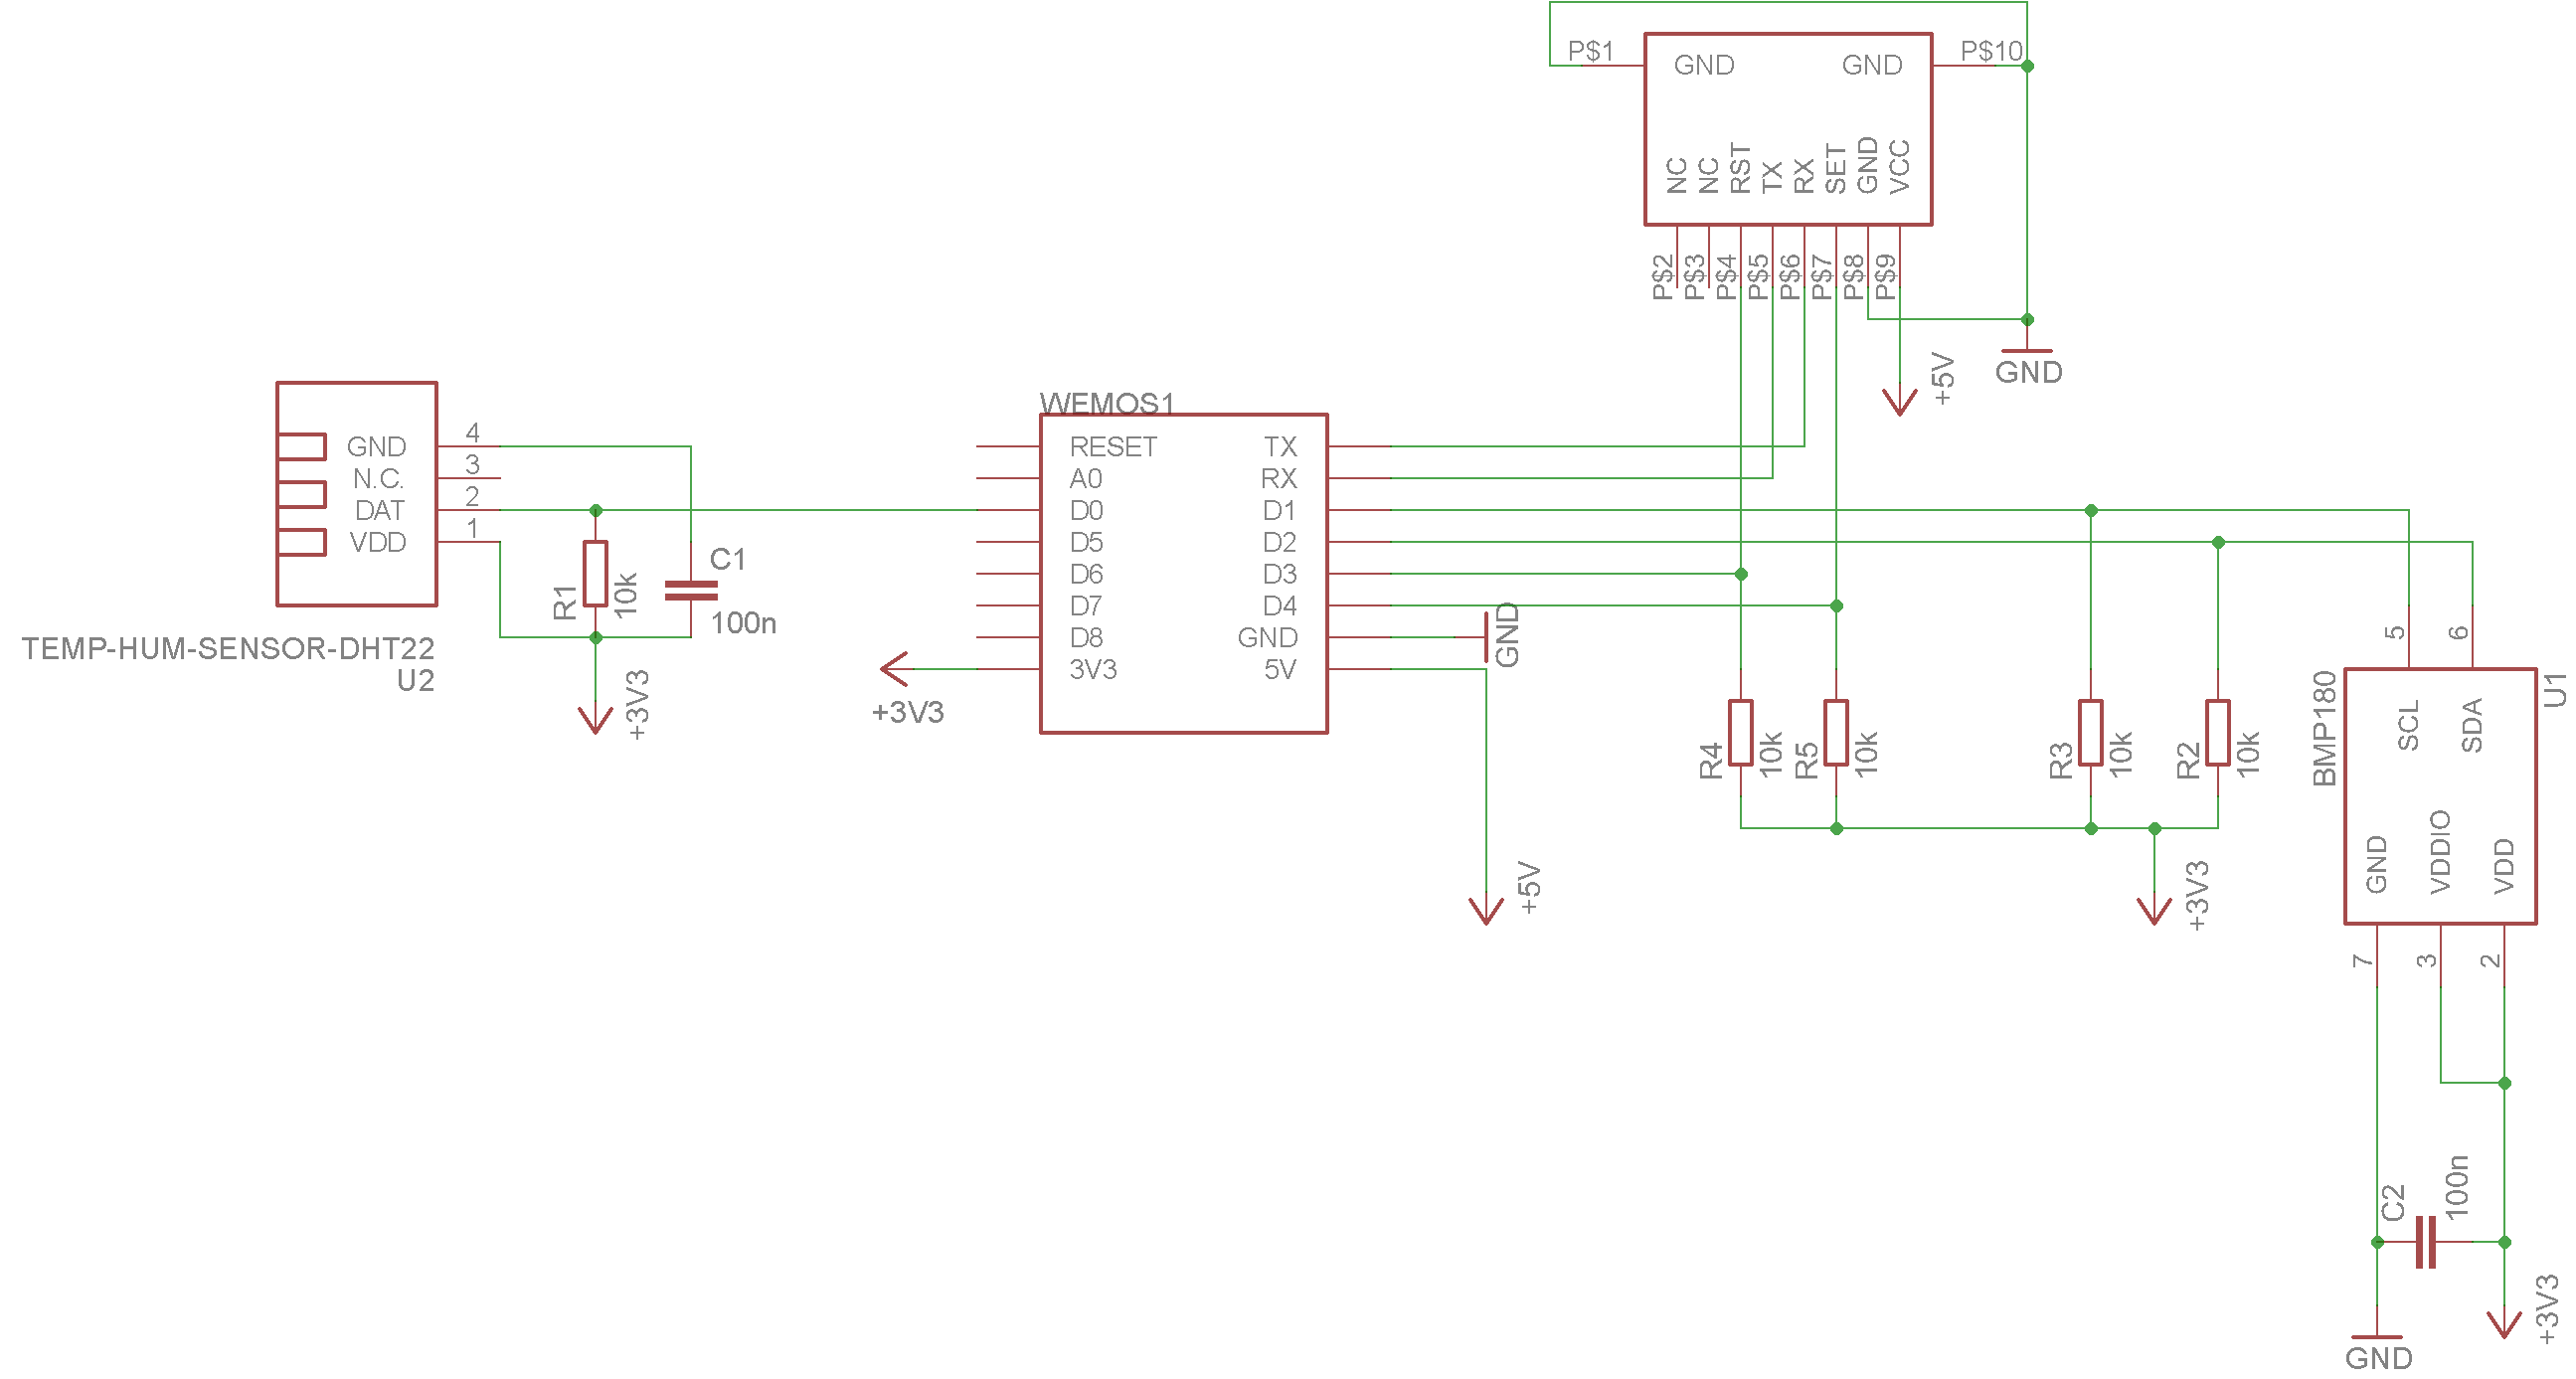
\includegraphics[width=\linewidth]{schematics.png}
				\caption{Schematics for the Air Pollution Sensor.}
				\label{fig:aps-schematics}
			\end{figure}
			
			Now that we know all the components (and their specifics) that have to be used in our device, we can make a detailed list of functions it has to perform:
			
			\begin{enumerate}
				\item An algorithm has to shut down and protect some of the sensors from extreme operating conditions (e.g. the PMS7003 sensor when the ambient temperature is below \SI{-10}{\celsius}).
				\item It has to take measurements of air pressure, temperature, and particulate matter concentration every minute.
				\item Since there are two temperature sensors available, an algorithm has to fall back to an operational sensor, if one of them fails. Otherwise, both sensors may be used in temperature measurement to reduce the value error.
				\item It has to be able to connect to several Wi-Fi Hotspots. The list of them will either have to be flashed with the firmware or made available through the cloud.
				\item Every five minutes, the device has to connect to a Wi-Fi hotspot and send the collected data to the cloud.
				\item There has to be a possibility to change the measurement and data transmission period through the cloud.
			\end{enumerate}
			
		\subsection{The Cloud}
			On the server side there would have to be implemented two several RESTful APIs. One for the Air Pollution Sensors (private API) and another one for the clients that use the graphical user interface (public API).
			The private API would have to feature several endpoints that would:
			\begin{itemize}
				\item Verify the authenticity of a device using its secret and access token pair through sha384 hash of a concatenation of client-server nonce pair and secret access token.
				\item Store the collected data in a database.
				\item Provide a device with useful weather data like wind speed for optimized sensor protection.
				\item Provide a confiugration for individual devices with parameters like sensor sampling period and data transmission period.
			\end{itemize}
			
		\subsection{Tasks Schedule}
			\resetrownum
			\begin{table}[h!]
				\begin{center}
					\caption{Schedule of the Tasks to be completed.}
					\label{tab:tasks-schedule}
					\begin{tabular}{l|p{5cm}|c}
						\textbf{No.} & \textbf{Task Description} & \textbf{Time Period} \\
						
						\hline
						\multicolumn{3}{c}{\textbf{Air Pollution Sensor}} \\
						\hline
						
						\rownum & Assemble the device on a breadboard and write a code to retrieve raw data from the sensors. Once we check that the device is operational we may continue onto the next step. & 21.10.19 -- 06.11.19 \\
						\rownum & Assemble the device on a prototype board. Test if the previously written code works. & 07.11.19 -- 08.11.19 \\
						\rownum & Develop and implement an algorithm to detect failure of one of the temperature sensors, a fall back in case of a failure and a way to decrease value error using measurement from two sensors. & 11.11.19 -- 13.11.19 \\
						\rownum & Develop and implement an algorithm to protect some of the sensors from exteme operating conditions & 14.11.19 -- 18.11.19 \\
						
						\hline
						\multicolumn{3}{c}{\textbf{Cloud}} \\
						\hline
						
						\rownum & Develop a database model and REST API that will be used by Air Pollution Sensors to upload the collected data and receive necessary commands. Implement the API using NodeJS and make use of it in the microcontroller firmware. & 19.11.19 -- 29.11.19 \\
						\rownum & Using the sketches of user interface, estimate the REST API endpoints necessary to implement to make it fully operational. Implement the API using NodeJS. &  02.12.19 -- 05.12.19 \\
						\rownum & Implement a user interface in ReactJS using the previously made sketches and client REST API. & 06.12.19 -- 20.12.19 \\
					\end{tabular}
				\end{center}
			\end{table}
			
			\begin{enumerate}
				\item Make an esp program that would fetch the necessary data from BMP180, DHT22 and PMS7003
				\item Develop hardware protection algorithm in case read operating conditions go out of normal operation conditions.
				\item Determine forgula for air pollution level.
			\end{enumerate}

	\newpage
	\bibliography{report} 
	\bibliographystyle{ieeetr}
		
\end{document}
